\documentclass[12pt,a4paper,titlepage]{scrartcl}

\usepackage{comment}
\usepackage[main=ngerman,english]{babel}
\usepackage[utf8]{inputenc}
\usepackage[T1]{fontenc}
\usepackage{lmodern}
\usepackage{geometry}
\geometry{left=2.5cm,right=2.5cm,top=2.5cm,bottom=3cm,head=29pt,foot=25pt}
\setlength{\footheight}{25pt}
\usepackage{microtype}
\usepackage{amsmath,amssymb,mathtools}
\numberwithin{equation}{section}
\numberwithin{table}{section}
\numberwithin{figure}{section}
\usepackage{siunitx}
\sisetup{locale=DE, separate-uncertainty=true, per-mode=fraction}
\usepackage{booktabs}
\usepackage{multirow}
\usepackage{graphicx}
\usepackage{float}
\usepackage{caption}
\usepackage{subcaption}
\usepackage[automark]{scrlayer-scrpage}
\usepackage[most]{tcolorbox}
\usepackage{hyperref}
\usepackage{pdfpages}
\usepackage{csvsimple-l3}
\usepackage{longtable}
\usepackage{graphicx}

\input{../../jupyterpackages.tex}


\newcommand{\pdfabbildung}[2]{%
    \refstepcounter{figure}%
    \addcontentsline{lof}{figure}{\protect\numberline{\thefigure}#1}%
    \label{#2}%
}

\newcommand{\pdftabelle}[2]{%
    \refstepcounter{table}%
    \addcontentsline{lot}{table}{\protect\numberline{\thetable}#1}%
    \label{#2}%
}


\hypersetup{colorlinks=true, linkcolor=blue!60!black, urlcolor=blue!60!black, citecolor=blue!60!black}

\clearpairofpagestyles

\chead{%
    \versuch\hfill\autor\\
    \rule{\textwidth}{0.2pt}%
}
\cfoot{%
    \rule{\textwidth}{0.2pt}\\[-0.5ex]
    \pagemark\ 
}
\addtokomafont{pagefoot}{\small}
\setlength{\parindent}{0pt}

\newtcolorbox{resultbox}[1][]{ 
    enhanced,
    colback=black!4!white,
    colframe=black!65!black,
    boxrule=0.8pt,
    arc=0.0mm,
    title=#1,
    fonttitle=\bfseries,
    %drop shadow
}


\newcommand{\versuch}{Versuch 25}
\newcommand{\titel}{Oszilloskop}
\newcommand{\praktikum}{Physikalisches Anfängerpraktikum 1}
\newcommand{\autor}{Jonathan Gießen}
\newcommand{\gruppe}{Gruppe 8}
\newcommand{\datum}{3. September 2026}
\newcommand{\betreuer}{Nick Rasberger}

\begin{document}

\pagestyle{scrheadings}

\begin{titlepage}



    \centering
    \vspace*{4cm}
    {\large Universität Heidelberg\par}
    {\small Fakultät für Physik und Astronomie\par}
    {\Large \praktikum\par}
    \vspace{0.8cm}
    {\LARGE \bfseries \versuch\ -- \titel\par}
    \vspace{1.5cm}

    \begin{tabular}{ll}
        \textbf{Autor:} & \autor\\
        \textbf{Gruppe:} & \gruppe\\
        \textbf{Betreuer:} & \betreuer\\
        \textbf{Versuchsdatum:} & \datum\\
    \end{tabular}

    \vfill
    \hrulefill\
\end{titlepage}

\tableofcontents

\bigskip
\begin{tcolorbox}[colback=gray!5,colframe=gray!60,boxrule=0.8pt,arc=0.01mm,title=KI-Hinweis]
    Für die sprachliche Formulierung dieses Protokolls wurde in Abschnitt \ref{Grundlagen} KI-gestützte Textgenerierung verwendet. 
\end{tcolorbox}
\clearpage
\section{Einleitung}
Das Oszilloskop ist ein unverzichtbares Werkzeug in der experimentellen Physik, das es ermöglicht, elektrische Signale in Echtzeit zu visualisieren und zu analysieren. In diesem Versuch werden wir die grundlegenden Funktionen eines Oszilloskops kennenlernen, einschließlich der Darstellung von Spannungsverläufen, der Messung von Frequenzen und Amplituden sowie der Untersuchung von Signalformen. Ziel ist es, ein tiefes Verständnis für die Bedienung des Geräts zu entwickeln und die gewonnenen Daten kritisch zu interpretieren.

Das Oszilloskop bietet die Möglichkeit, sowohl zeitabhängige als auch frequenzabhängige Eigenschaften von Signalen zu untersuchen. Durch die Anwendung verschiedener Messmethoden und -techniken werden wir das Gerät in unterschiedlichen Szenarien einsetzen, um die Vielseitigkeit und Präzision des Oszilloskops zu demonstrieren. Die gewonnenen Erkenntnisse werden nicht nur die theoretischen Grundlagen der Signalverarbeitung vertiefen, sondern auch praktische Fähigkeiten im Umgang mit modernen Messinstrumenten fördern.

In diesem Versuch wird ein digitales Speicheroszilloskop verwendet (Tektronix TBS1072B), das eine Bandbreite von 70 MHz und eine Abtastrate von 1 GS/s bietet.

Im ersten Teil werden verschiedene Signalformen, wie Sinuswellen, Aufladekurven eines Kondensator und Pulsweitenmodulationen untersucht und ihre Kenngrößen, wie Amplitude, Frequen, Spitze-Spitze-Spannung und Gleichspannungsanteil bestimmt und analysiert
Danach wird mit Hilfe des Oszilloskops und der Fourier-Analyse die Frequenzspektren von komplexen Schwebungssignalen untersucht. 
Zum Abschluss wird die Kabellänge eines Coaxialkabels mit Hilfe der Laufzeitmessung bestimmt.


\section{Grundlagen und Theorie}\label{Grundlagen}
\paragraph{Frequenz $f$}
Die Frequenz $f$ eines periodischen Signals ist mit die charakteristische Größe, die als die Anzahl der Schwingungen pro Zeiteinheit definiert wird. Sie wird in Hertz (Hz) gemessen und ist der Kehrwert der Periodendauer $T$:
\begin{equation}
    f = \frac{1}{T}
\end{equation}
Die Frequenz ist ein entscheidender Parameter, der die zeitliche Struktur eines Signals beschreibt und in vielen Anwendungen, von der Kommunikationstechnik bis zur Signalverarbeitung, eine zentrale Rolle spielt. Bei Schallwellen bestimmt die Freuquenz den Tonhöhenbereich, während sie bei elektromagnetischen Wellen die Art der Strahlung charakterisiert. Verschiedene Freuqenzen bei Lichtwellen entsprechen unterschiedlichen Farben, während bei Radiowellen die Frequenz die Übertragungsbandbreite und Reichweite beeinflusst. Die präzise Messung und Analyse der Frequenz ist daher von großer Bedeutung in der Physik und Technik.

\paragraph{Periodendauer $T$}
Die Periodendauer $T$ eines periodischen Signals ist die Zeit, die für eine vollständige Schwingung oder einen Zyklus benötigt wird. Sie ist der Kehrwert der Frequenz $f$ und wird in Sekunden (s) gemessen:
\begin{equation}
    T = \frac{1}{f}
\end{equation}

\paragraph{Wellenlänge $\lambda$}
Die Wellenlänge $\lambda$ ist die räumliche Länge einer vollständigen Schwingung oder eines Zyklus einer Welle. Sie wird in Metern (m) gemessen und ist mit der Frequenz $f$ und der Ausbreitungsgeschwindigkeit $v$ der Welle verknüpft:
\begin{equation}
    \lambda = \frac{v}{f}
\end{equation}
Bei Veränderung der Ausbreitungsgeschwindigkeit bleibt die Frequenz erhalten, die Wellenlänge ändert sich jedoch entsprechend. Dies ist besonders relevant bei der Betrachtung von Wellen, die sich in unterschiedlichen Medien ausbreiten, da die Ausbreitungsgeschwindigkeit von den physikalischen Eigenschaften des Mediums abhängt.

\paragraph{Ausbreitungsgeschwindigkeit $v$}
Die Ausbreitungsgeschwindigkeit $v$ ist die Geschwindigkeit, mit der sich eine Welle durch ein Medium bewegt. Sie hängt von den physikalischen Eigenschaften des Mediums ab und wird in Metern pro Sekunde (m/s) gemessen. Für elektromagnetische Wellen lässt sich aus dem Maxwellschen Gleichungssystem ableiten, dass für die Ausbreitungsgeschwindigkeit im Vakuum ($\epsilon_r = 1{,}\ \mu_r = 1$) gilt:
\begin{equation}
    v = c = \frac{1}{\sqrt{\mu_0 \mu_r \epsilon_0 \epsilon_r}} \approx 3 \cdot 10^8 \frac{\text{m}}{\text{s}}
\end{equation}

\paragraph{Phase $\varphi$}
Die Phase $\varphi$ ist ein Maß für die Position eines Punktes in einem periodischen Prozess. Sie wird in Radiant (rad) oder Grad (°) gemessen und beschreibt den zeitlichen Versatz einer Welle im Vergleich zu einem Referenzzeitpunkt. Die Phase ist besonders wichtig bei der Analyse von Wellen, da sie den Zusammenhang zwischen verschiedenen Wellen beschreibt und bei der Interferenz von Wellen eine entscheidende Rolle spielt.

In der Wellengleichung wird die Phase $\varphi$ oft als Argument der Sinus- oder Kosinusfunktion verwendet, um die zeitliche Entwicklung der Welle zu beschreiben. Eine Phasenverschiebung kann durch unterschiedliche Wege, Medien oder Quellen verursacht werden und beeinflusst die Überlagerung von Wellen, was zu konstruktiver oder destruktiver Interferenz führen kann.

\paragraph{Amplitude $A$}
Die Amplitude $A$ ist die maximale Auslenkung einer Welle von ihrer Ruhelage. Sie wird in der Regel in Volt (V) für elektrische Signale oder in Metern (m) für mechanische Wellen gemessen. Die Amplitude ist ein Maß für die Energie, die eine Welle transportiert, und spielt eine entscheidende Rolle bei der Charakterisierung von Signalen. In der Signalverarbeitung wird die Amplitude oft verwendet, um die Stärke eines Signals zu quantifizieren und zu analysieren.
\begin{figure}
    \centering
    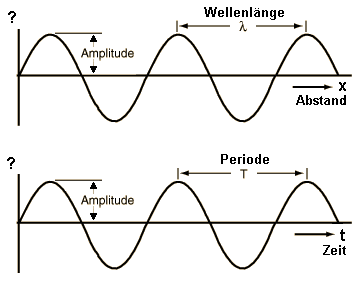
\includegraphics[width=0.6\textwidth]{img/Wellencharakter.png}
    \caption{Darstellung der verschiedenen Kenngrößen einer Welle}
    \footnotemark
    \label{fig:amplitude}
\end{figure}
\footnotetext{Quelle: \url{https://sengpielaudio.com/WellenSinusZeitAbstandTime.gif}}

\paragraph{Spitzen-Spitzen-Spannung $U_{pp}$}
Die Spitzen-Spitzen-Spannung $U_{pp}$ ist die Differenz zwischen dem höchsten und dem niedrigsten Punkt eines periodischen Signals. Sie wird in Volt (V) gemessen und ist ein Maß für die maximale Amplitude des Signals. Die Spitzen-Spitzen-Spannung ist besonders relevant bei der Analyse von Wechselspannungen, da sie die gesamte Spannungsdynamik eines Signals beschreibt und in vielen Anwendungen, wie der Signalübertragung und -verarbeitung, eine wichtige Rolle spielt.
\begin{equation}
    U_{pp} = 2 \cdot A_U = U_{max} - U_{min}\label{eq:spitzen_spitzen_spannung}
\end{equation}

\paragraph{Wellenwiderstand und Reflexion auf einer Leitung}
Der Wellenwiderstand $Z$ ist ein Maß für den Widerstand, den eine Leitung einer Welle entgegensetzt. Er wird in Ohm ($\Omega$) gemessen und hängt von den physikalischen Eigenschaften der Leitung ab, wie dem Material, der Geometrie und der Frequenz des Signals.

Er berechnet sich aus der Induktivität $L$ und der Kapazität $C$ der Leitung:
\begin{equation}
    Z = \sqrt{\frac{L}{C}}
\end{equation}

\textbf{Reflexion auf einer Leitung:} Breitet sich ein elektrisches Signale entlang
einer Leitung aus so können diese an den Änderungen des Wellenwiderstands reflektiert werden. Das passiert vor allem am Ende der Leitung, je nachdem wie
die Leitung abgeschlossen ist. Betrachtet man einzelne Pulse auf einer Leitung, je nach die Art des Abschlusses der Leitung, so werden diese unterschiedlich reflektiert.
Treffen diese auf ein offenes Leitungsende so werden diese hier ohne Phasensprung reflektiert und laufen zurück zum Sender (Reflexion am offenen Ende).
Ist dagegen das Leitungsende kurzgeschlossen so werden die Impulse mit einem
Phasensprung reflektiert. Der zurücklaufende Impuls hat die umgekehrte Polarität wie die hinlaufende Welle (Reflexion am festen Ende). \cite{PAPskript}

\paragraph{Fourier-Analyse}
Die Fourier-Analyse ist eine mathematische Methode zur Zerlegung von Signalen in ihre Frequenzkomponenten. Sie basiert auf der Idee, dass jedes periodische Signal als Summe von Sinus- und Kosinusfunktionen unterschiedlicher Frequenzen dargestellt werden kann. Die Fourier-Analyse ermöglicht es, die Frequenzstruktur eines Signals zu untersuchen und die Amplituden und Phasen der einzelnen Frequenzkomponenten zu bestimmen. Sie ist ein unverzichtbares Werkzeug in der Signalverarbeitung, der Kommunikationstechnik und vielen anderen Bereichen der Physik und Technik. Durch die Anwendung der Fourieraufteilung können komplexe Signale in ihre Grundfrequenzen zerlegt werden, was eine detaillierte Analyse und Interpretation der Signalcharakteristika ermöglicht.

\paragraph{Pulsweitenmodulation (PWM)}
Um moderene LEDs zu dimmen oder Motoren zu steuern, wird häufig die Pulsweitenmodulation (PWM) eingesetzt. Bei der PWM wird die Leistung eines Signals durch die Variation der Pulsbreite gesteuert, während die Frequenz konstant bleibt. Dies ermöglicht eine effiziente Steuerung von elektrischen Geräten, da die Energieübertragung in diskreten Pulsen erfolgt, anstatt kontinuierlich. Die PWM-Technik ist besonders vorteilhaft in Anwendungen, bei denen eine präzise Steuerung der Leistung erforderlich ist, wie z.B. in der Beleuchtungstechnik, der Motorsteuerung und der digitalen Signalverarbeitung. Sie bietet einfachere Aufbauten wie bei der analogen Steuerung und ermöglicht eine höhere Effizienz und Flexibilität in der Leistungsregelung. Mikrocontroller können die PWM-Signale einfach erzeugen, indem sie digitale Ausgänge mit variabler Pulsbreite steuern, was die Integration in moderne elektronische Systeme erleichtert, während analoge Steuerungen oft komplexere Schaltungen erfordern.
\begin{figure}
    \centering
    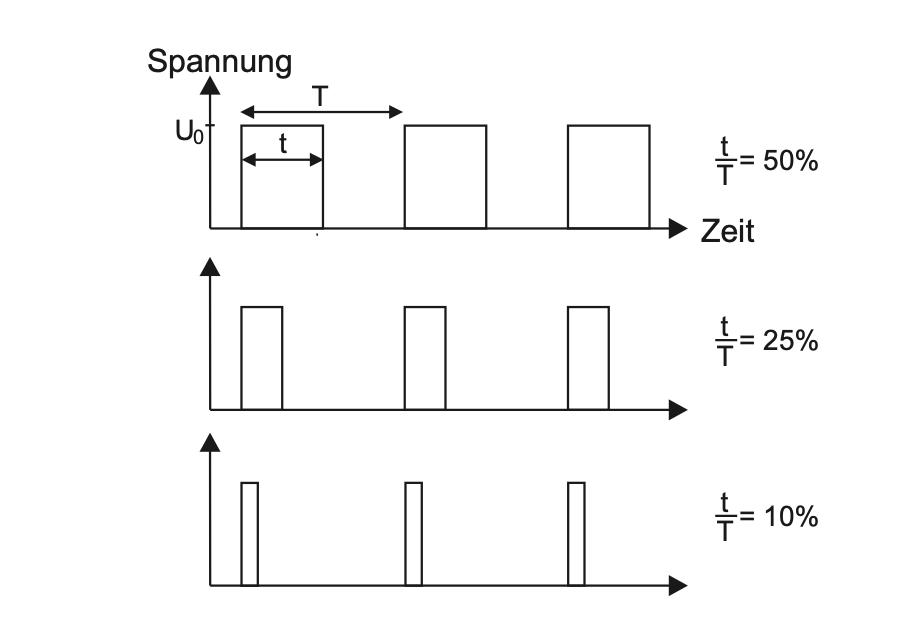
\includegraphics[width=0.6\textwidth]{img/PWM.png}
    \caption{Darstellung der Pulsweitenmodulation (PWM) mit unterschiedlichen Tastverhältnissen.}\cite{PAPskript}

    \label{fig:pwm}
\end{figure}

Der Mittelwert eines PWM-Signals kann durch das Tastverhältnis $D$ = $\frac{t}{T}$ berechnet werden:
\begin{equation}
    U_{PWM} = D \cdot U_{max}\label{PWMMittelwert}
\end{equation}  

Die Effektivspannung eines PWM-Signals kann mit folgender Formel berechnet werden:
\begin{equation}
    U_{eff} = \sqrt{D} \cdot U_{max}\label{PWMEffektiv}
\end{equation}

\section{Messprotokoll}

\subsection{Versuchsaufbau und Aufgaben}
Im folgenden Abschnitt werden die Aufgaben und der Versuchsaufbau beschrieben, die im Rahmen des Oszilloskop-Versuchs durchgeführt wurden. Der Versuchsaufbau besteht aus einem digitalen Speicheroszilloskop (Tektronix TBS1072B), das mit verschiedenen Signalquellen verbunden ist, um unterschiedliche Signalformen zu erzeugen und zu analysieren. 

\begin{itemize}
    \item \textbf{Aufgabe 1.1:} Untersuchung verschiedener Signalformen, einschließlich Sinuswellen, Aufladekurven eines Kondensators und Pulsweitenmodulationen. Bestimmung und Analyse der Kenngrößen: Amplitude, Frequenz, Spitze-Spitze-Spannung und Gleichspannungsanteil.
    \item \textbf{Aufgabe 1.2:} Analyse der Frequenzspektren von Schwebungssignalen mithilfe des Oszilloskops und der Fourier-Analyse.
    \item \textbf{Aufgabe 2:} Bestimmung von Periode, Pulsbreite, Pulshöhe, Effektivspannung und Mittelwert von PWM-Signalen auf eine LED - Untersuchung der Auswirkungen unterschiedlicher Tastverhältnisse auf die LED-Helligkeit.
    \item \textbf{Aufgabe 3:} Bestimmung der Kabellänge eines Coaxialkabels durch Laufzeitmessung. Untersuchung der Reflexionen an offenen, kurzgeschlossenen und mit einem Potentiometer versehenen Leitungsenden, um die Auswirkungen auf die Signalübertragung zu analysieren. Durch verstellen des Potentiometers wird der Wellenwiderstand der Leitung bestimmt und die Reflexionen minimiert.
\end{itemize}

\pdfabbildung{Messaufbau}{fig:messprotokoll-1}
\pdfabbildung{Signal 1}{fig:messprotokoll-2}
\pdfabbildung{Signal 2}{fig:messprotokoll-3}
\pdfabbildung{Signal 3}{fig:messprotokoll-4}
\pdfabbildung{Schwebung FFT}{fig:messprotokoll-5}
\pdfabbildung{Schwebung}{fig:messprotokoll-6}
\pdfabbildung{PWM-Signal}{fig:messprotokoll-7}
\pdftabelle{Tabelle der Messungen PWM}{tbl:MessungenA2}
\pdfabbildung{Generiertes Signal für Messung von Kabellänge}{fig:messprotokoll-8}
\pdfabbildung{Reflektiertes Signal(Offenes Ende)}{fig:messprotokoll-9}
\pdfabbildung{Reflektiertes Signal(Kurzgeschlossenes Ende)}{fig:messprotokoll-10}


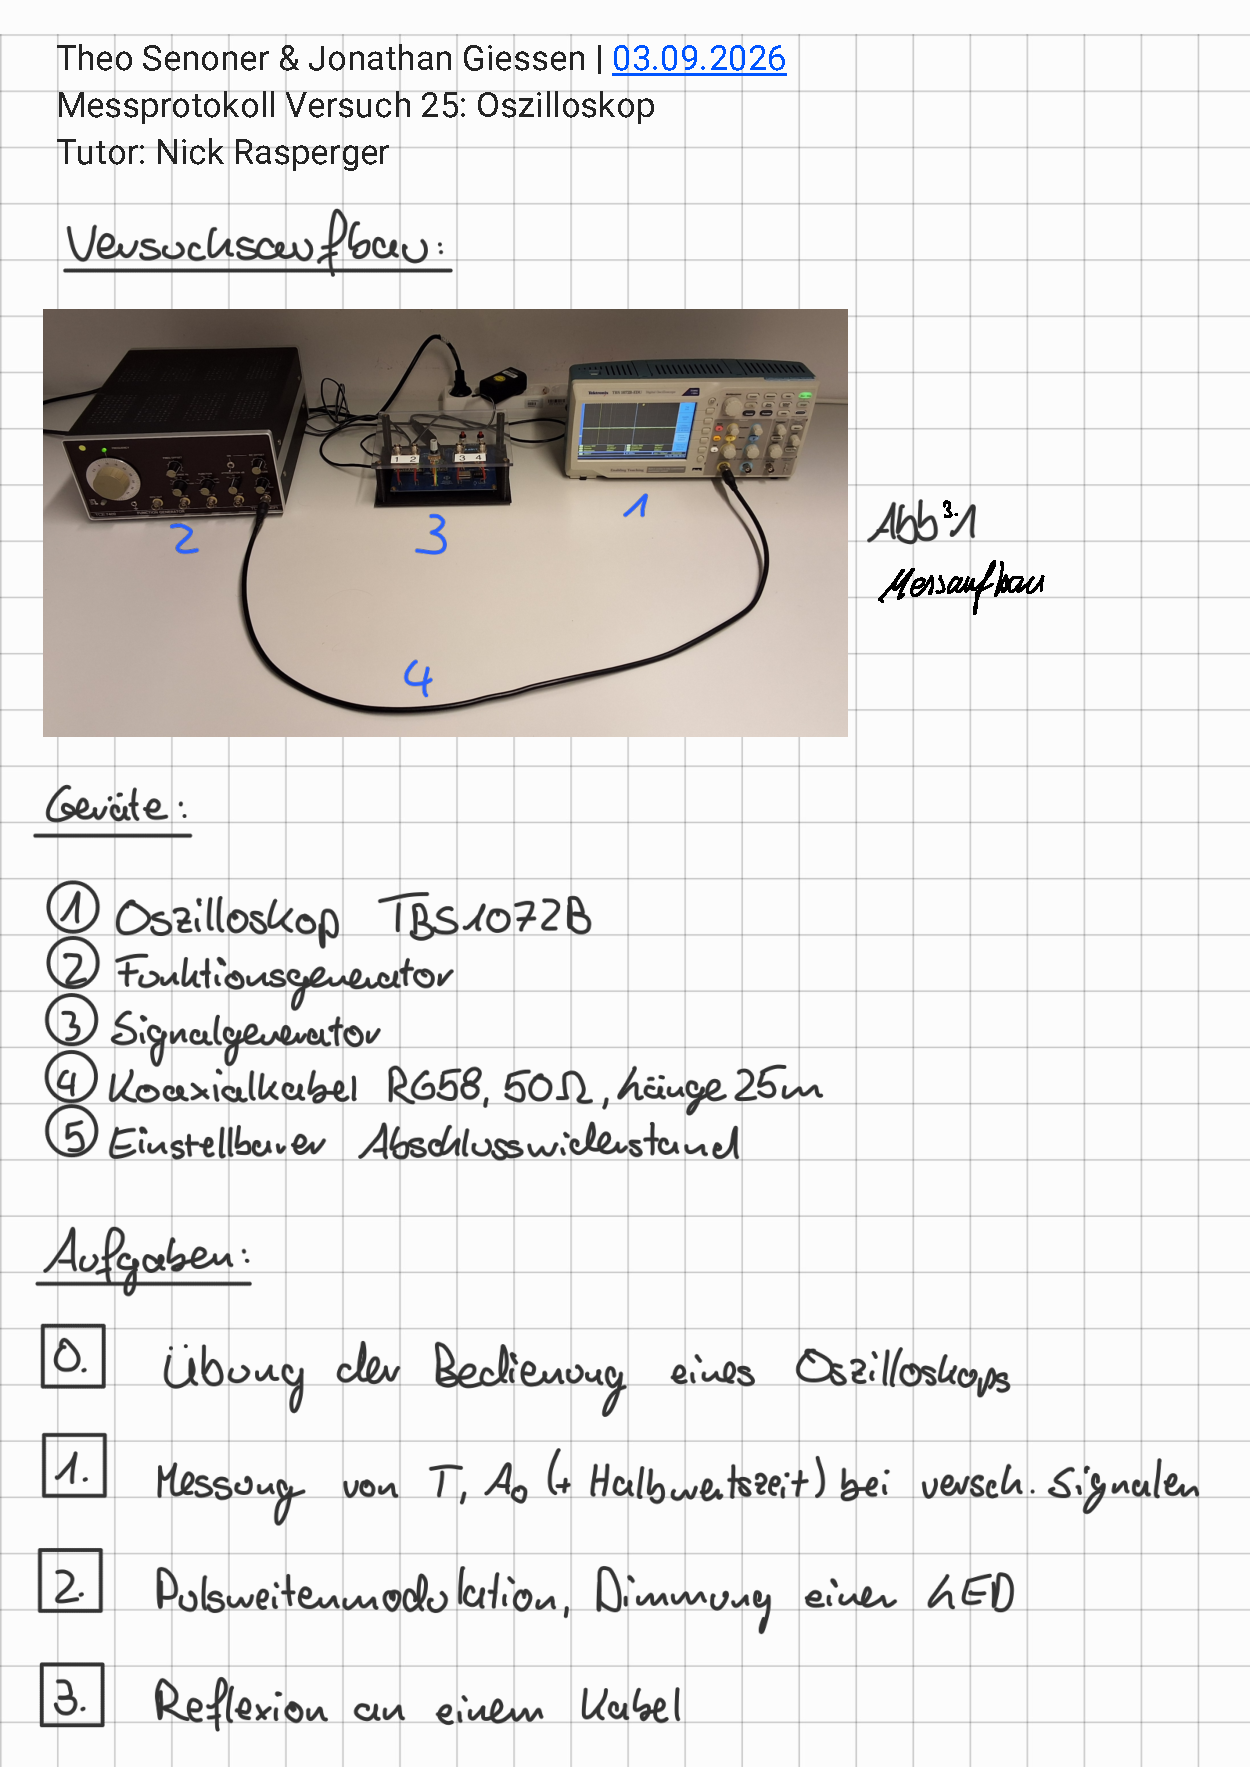
\includepdf[
    pages=-,
    width=\textwidth,
    height=\textheight,
    keepaspectratio,
    pagecommand={\thispagestyle{scrheadings}}
]{../Messprotokoll 25.pdf}

\section{Auswertung}
\subsection{Aufgabe 1: Berechnung der Schwebungsfrequenzen}
Gemäß der Aufgabenstellung werden aus den im Frequenzspektrum gemessenen Einzelfrequenzen $f_I$ und $f_{II}$ (mit $f_{II} > f_I$) die Größen $f_1$ (mittlere Trägerfrequenz) und $f_2$ (Modulationsfrequenz der Einhüllenden) berechnet:
\begin{equation}
    f_1 = \frac{f_{II} + f_I}{2}, \qquad f_2 = \frac{f_{II} - f_I}{2}
\end{equation}

\medskip
Aus dem Messprotokoll (FFT-Spektrum, Abbildung \ref{fig:messprotokoll-5}) entnehmen wir:
\begin{itemize}
    \item $f_I = (1.395 \pm 0.005)\,\text{kHz} = (1395 \pm 5)\,\text{Hz}$
    \item $f_{II} = (1.580 \pm 0.005)\,\text{kHz} = (1580 \pm 5)\,\text{Hz}$
\end{itemize}

Nach der Gaußschen Fehlerfortpflanzung gilt für beide theoretischen Größen dieselbe Unsicherheit:
\begin{equation}
    \begin{aligned}
        \Delta{f_{1,2}} &= \sqrt{\left(\frac{\partial f_{1,2}}{\partial f_I}\right)^2 \Delta{f_I}^2 + \left(\frac{\partial f_{1,2}}{\partial f_{II}}\right)^2 \Delta{f_{II}}^2} \\
        &= \frac{1}{2} \sqrt{(5\,\text{Hz})^2 + (5\,\text{Hz})^2} = \frac{5}{\sqrt{2}}\,\text{Hz} \approx 3.54\,\text{Hz} \approx 4\,\text{Hz}
    \end{aligned}
\end{equation}

Damit ergeben sich die theoretisch berechneten Referenzwerte zu:
\begin{align*}
    f_1 &= \frac{1580\,\text{Hz} + 1395\,\text{Hz}}{2} = 1487.5\,\text{Hz} \approx (1488 \pm 4)\,\text{Hz} \\
    f_2 &= \frac{1580\,\text{Hz} - 1395\,\text{Hz}}{2} = 92.5\,\text{Hz} \approx (93 \pm 4)\,\text{Hz}
\end{align*}

\begin{resultbox}[Ergebnis der theoretischen Berechnung]
    Die aus den Spektralfrequenzen berechneten Größen lauten:
    \begin{align*}
        f_1 &= (1488 \pm 4)\,\text{Hz} = (1.488 \pm 0.004)\,\text{kHz}, \\
        f_2 &= (93 \pm 4)\,\text{Hz}.
    \end{align*}
\end{resultbox}

\medskip
\textbf{Vergleich und Korrektur mit der Cursor-Messung im Zeitbereich:}

Im Messprotokoll (Signal 4) wurde für die schnelle Schwingung über 10 Perioden gemessen:
\begin{equation*}
    f_{1,\text{mess}} = (1572 \pm 15)\,\text{Hz}
\end{equation*}

Für die Schwebung wurde am Oszilloskop ein Zeitintervall von $T_{S,3} = (15.00 \pm 0.06)\,\text{ms}$ abgelesen, woraus zunächst $f_S = 66.67\,\text{Hz}$ berechnet wurde. Abbildung \ref{fig:messprotokoll-6} zeigt die Überprüfung des Signals bei einer Zeitbasis von $2.50\,\text{ms/Div}$, wobei dieses Zeitintervall genau $N = 3$ Schwebungsbäuchen entspricht. 

Die tatsächliche Periodendauer eines einzelnen Bauchs beträgt somit:
\begin{equation}
    T_{\text{Bauch}} = \frac{T_{S,3}}{3} = \frac{15.00\,\text{ms}}{3} = (5.000 \pm 0.020)\,\text{ms}
\end{equation}
Daraus folgt für die experimentelle Frequenz der Schwebungsbäuche $f_{\text{Bauch}}$:
\begin{equation}
    f_{\text{Bauch}} = \frac{1}{T_{\text{Bauch}}} = 3 \cdot f_S = 3 \cdot 66.67\,\text{Hz} = (200.0 \pm 0.8)\,\text{Hz}
\end{equation}

Da ein Schwebungsbauch einer Halbperiode der Einhüllenden entspricht, gilt für die zu $f_2$ analoge Modulationsfrequenz $f_{2,\text{korr}} = \frac{f_{\text{Bauch}}}{2}$:
\begin{equation}
    f_{2,\text{korr}} = \frac{200.0\,\text{Hz}}{2} = (100.0 \pm 0.4)\,\text{Hz}
\end{equation}

\medskip
\textbf{Statistischer Vergleich und $\sigma$-Abweichungen:}

Zur quantitativen Beurteilung der Übereinstimmung wird die Differenz $d = |f_{\text{mess}} - f_{\text{ber}}|$ im Verhältnis zur kombinierten Unsicherheit $\Delta{\text{ges}} = \sqrt{\Delta{\text{mess}}^2 + \Delta{\text{ber}}^2}$ betrachtet:

\begin{itemize}
    \item \textbf{Schwingungsfrequenz $f_1$:}
    \begin{align*}
        d_1 &= |1572\,\text{Hz} - 1487.5\,\text{Hz}| = 84.5\,\text{Hz} \approx 84\,\text{Hz} \quad (\approx 5.7\,\%) \\
        \Delta{\text{ges},1} &= \sqrt{(15\,\text{Hz})^2 + (3.54\,\text{Hz})^2} \approx 15.4\,\text{Hz} \\
        \frac{d_1}{\Delta{\text{ges},1}} &= \frac{84.5\,\text{Hz}}{15.4\,\text{Hz}} \approx 5.5\,\sigma
    \end{align*}
    
    \item \textbf{Modulationsfrequenz $f_2$:}
    \begin{align*}
        d_2 &= |100.0\,\text{Hz} - 92.5\,\text{Hz}| = 7.5\,\text{Hz} \quad (\approx 8.1\,\%) \\
        \Delta{\text{ges},2} &= \sqrt{(0.4\,\text{Hz})^2 + (3.54\,\text{Hz})^2} \approx 3.56\,\text{Hz} \\
        \frac{d_2}{\Delta{\text{ges},2}} &= \frac{7.5\,\text{Hz}}{3.56\,\text{Hz}} \approx 2.1\,\sigma
    \end{align*}
\end{itemize}

\begin{resultbox}
    
    \textbf{Ergebnis der statistischen Analyse:}
    \begin{itemize}
        \item Die Schwingungsfrequenz $f_1$ weicht um $5.5\,\sigma$ von der theoretischen Berechnung ab, was auf eine signifikante Diskrepanz hinweist.
        \item Die Modulationsfrequenz $f_2$ weicht um $2.1\,\sigma$ von der theoretischen Berechnung ab, was auf eine moderate Abweichung hinweist.
    \end{itemize}
\end{resultbox}
\medskip


\subsection{Aufgabe 2: Berechnung der Mittel- und Effektivwerte von PWM-Signalen}
Für ein ideales Rechteck- bzw. PWM-Signal mit Periodendauer $T$, Pulsbreite $\tau$ und Pulshöhe $U_0$ ergeben sich der lineare Mittelwert $\overline{U}$ und der Effektivwert $U_{\text{eff}}$ aus Gleichung \ref{PWMMittelwert} und \ref{PWMEffektiv}:
\begin{equation}
    \overline{U} = \frac{\tau}{T} \cdot U_0, \qquad U_{\text{eff}} = \sqrt{\frac{\tau}{T}} \cdot U_0
\end{equation}

Nach der Gaußschen Fehlerfortpflanzung lauten die Unsicherheiten für beide Größen:
\begin{align}
    \Delta{\overline{U}} &= \overline{U} \cdot \sqrt{\left(\frac{\Delta\tau}{\tau}\right)^2 + \left(\frac{\Delta T}{T}\right)^2 + \left(\frac{\Delta U_0}{U_0}\right)^2} \\
    \Delta{U_{\text{eff}}} &= U_{\text{eff}} \cdot \sqrt{\frac{1}{4}\left(\frac{\Delta\tau}{\tau}\right)^2 + \frac{1}{4}\left(\frac{\Delta T}{T}\right)^2 + \left(\frac{\Delta U_0}{U_0}\right)^2}
\end{align}

Es fällt auf, dass bei verschieden langen Pulsen die angeschlossene LED dunkel bzw. hell leuchtet. Die Messwerte für die beiden Zustände „Dunkel“ und „Hell“ sind in Tabelle \ref{tbl:MessungenA2} im Messprotokoll zusammengefasst.
\paragraph{1. Zustand „Dunkel“:}
Mit $T = (1.02 \pm 0.10)\,\text{ms}$, $\tau = (0.30 \pm 0.10)\,\text{ms}$ und $U_0 = (3.52 \pm 0.04)\,\text{V}$:
\begin{align}
    \overline{U}_{\text{ber}} &= \frac{0.30\,\text{ms}}{1.02\,\text{ms}} \cdot 3.52\,\text{V} = 1.035\,\text{V} \pm 0.360\,\text{V} \approx (1.0 \pm 0.4)\,\text{V} \\
    U_{\text{eff,ber}} &= \sqrt{\frac{0.30\,\text{ms}}{1.02\,\text{ms}}} \cdot 3.52\,\text{V} = 1.909\,\text{V} \pm 0.332\,\text{V} \approx (1.9 \pm 0.4)\,\text{V}
\end{align}

\paragraph{2. Zustand „Hell“:}
Mit $T = (1.02 \pm 0.10)\,\text{ms}$, $\tau = (0.82 \pm 0.10)\,\text{ms}$ und $U_0 = (3.52 \pm 0.04)\,\text{V}$:
\begin{align}
    \overline{U}_{\text{ber}} &= \frac{0.82\,\text{ms}}{1.02\,\text{ms}} \cdot 3.52\,\text{V} = 2.830\,\text{V} \pm 0.444\,\text{V} \approx (2.8 \pm 0.5)\,\text{V} \\
    U_{\text{eff,ber}} &= \sqrt{\frac{0.82\,\text{ms}}{1.02\,\text{ms}}} \cdot 3.52\,\text{V} = 3.156\,\text{V} \pm 0.248\,\text{V} \approx (3.16 \pm 0.25)\,\text{V}
\end{align}

$\Delta_\text{ges}$ berechnet sich wieder aus der Gaußschen Fehlerfortpflanzung:
\begin{align}
    \Delta{\text{ges}} &= \sqrt{\Delta{\text{ber}}^2 + \Delta{\text{mess}}^2}\\
    \Delta_{\text{ges,Dunkel}} &= \sqrt{0.4^2 + 0.01^2}\,\text{V} \approx 0.4\,\text{V}\\
    \Delta_{\text{ges,Hell}} &= \sqrt{0.5^2 + 0.01^2}\,\text{V} \approx 0.5\,\text{V}\\
    \Delta_{\text{ges,Hell,eff}} &= \sqrt{0.25^2 + 0.01^2}\,\text{V} \approx 0.25\,\text{V}
\end{align}

\begin{resultbox}[Ergebnis]

        \begin{tabular}{lccccc}
            Zustand & Größe & Berechnet & Gemessen & Abweichung $d$ & $d/\Delta{\text{ges}}$ \\
            \midrule
            Dunkel & $\overline{U}$ & $(1.0 \pm 0.4)\,\text{V}$ & $(1.260 \pm 0.010)\,\text{V}$ & $0.3\,\text{V}$ & $0.6\,\sigma$ \\
            Dunkel & $U_{\text{eff}}$ & $(1.91 \pm 0.4)\,\text{V}$ & $(1.900 \pm 0.010)\,\text{V}$ & $0.01\,\text{V}$ & $0.03\,\sigma$ \\
            \midrule
            Hell & $\overline{U}$ & $(2.8 \pm 0.5)\,\text{V}$ & $(2.660 \pm 0.010)\,\text{V}$ & $0.1\,\text{V}$ & $0.3\,\sigma$ \\
            Hell & $U_{\text{eff}}$ & $(3.16 \pm 0.25)\,\text{V}$ & $(3.140 \pm 0.010)\,\text{V}$ & $0.02\,\text{V}$ & $0.08\,\sigma$ \\
            \bottomrule
        \end{tabular}

\end{resultbox}


\subsection {Aufgabe 3: Bestimmung der Kabellänge eines Coaxialkabels}
Die Kabellänge $l$ eines Coaxialkabels kann durch die Laufzeitmessung bestimmt werden. Uns ist bekannt, dass die Ausbreitungsgeschwindigkeit im Kabel des Typs RG58 66\% der Lichtgeschwindigkeit $c$ beträgt. Die Laufzeit $\Delta t$ eines Signals durch das Kabel wird mit dem Oszilloskop gemessen, und die Ausbreitungsgeschwindigkeit $v$ des Signals im Kabel wird durch die Materialeigenschaften des Coaxialkabels bestimmt. Für einen Weg im Kabel gilt die Beziehung: 

\begin{equation}
    l = v \cdot \Delta \tau
\end{equation}
Da das Signal im Kabel hin und zurück läuft, muss die gemessene Laufzeit $\Delta t$ durch 2 geteilt werden, um die effektive Kabellänge zu berechnen:
\begin{equation}
    l = \frac{v \cdot \Delta \tau}{2}\label{Kabellänge}
\end{equation}
Die Unsicherheit in der Kabellänge $\Delta l$ ergibt sich aus der Unsicherheit in der Laufzeitmessung $\Delta \tau$ und der Unsicherheit in der Ausbreitungsgeschwindigkeit $\Delta v$\footnote{Für den gegebenen Weet der Ausbreitungsgeschwindigkeit $v$ wiurde keine Unsicherheit vorgegeben}:
\begin{equation}
    \Delta l = \sqrt{\left(\frac{v \cdot \Delta \tau}{2}\right)^2 + \left(\frac{\Delta v \cdot \Delta \tau}{2}\right)^2}\label{KabellängeUnsicherheit}
\end{equation}  

Die gegebenen\ Werte betragen:
\begin{table}
    \centering
    \caption{Messwerte für die Berechnung der Kabellänge}
    \begin{tabular}{c|c}
        \toprule
        Größe & Wert\\
        \midrule
        Laufzeit $\Delta t$ & $(248.0 \pm 2.0)\,\text{ns}$ \\
        Ausbreitungsgeschwindigkeit $v$ & $(0.66 \cdot c = 1.98 \cdot 10^8)\,\text{m/s}$ \\
        Widerstand $Z$ & $(62.1 \pm 0.3)\,\Omega$ \\
        \bottomrule
    \end{tabular}
\end{table}

Mit diesen Werten in Gleichung \ref{Kabellänge} und \ref{KabellängeUnsicherheit} eingesetzt, ergibt sich die Kabellänge zu:
\begin{equation}
    l = \frac{1.98 \cdot 10^8\,\text{m/s} \cdot 248.0 \cdot 10^{-9}\,\text{s}}{2} \approx 24.55\,\text{m}
\end{equation}
Die Unsicherheit in der Kabellänge beträgt:

\begin{equation}
    \Delta l = \sqrt{\left(\frac{1.98 \cdot 10^8\,\text{m/s} \cdot 2.0 \cdot 10^{-9}\,\text{s}}{2}\right)^2} = 0.198\,\text{m} \approx 0.20\,\text{m}
\end{equation}  

Der Literaturwert für die Kabellänge beträgt $l_\text{lit} = 25\,\text{m}$, was eine eine Sigma Abweichung von:
\begin{equation}
    \sigma = \frac{|l - l_\text{lit}|}{\Delta l} = \frac{|24.55\,\text{m} - 25\,\text{m}|}{0.20\,\text{m}} \approx 2.25\,\sigma
\end{equation}

ergibt.

\subsection{Vergleich des Abschlusswiderstands mit dem Wellenwiderstand}
Am Koaxialkabel vom Typ RG58 wurde der einstellbare Abschlusswiderstand so justiert, dass am Leitungsende keine Reflexion mehr auftrat (reflexionsfreier Leitungsabschluss). Der am Potentiometer gemessene Widerstandswert sowie der nominelle Wellenwiderstand des Kabels lauten:
\begin{align*}
    R_0 &= (62.1 \pm 0.3)\,\Omega \\
    Z_0 &= 50\,\Omega \quad (\text{Herstellerangabe RG58})
\end{align*}

\paragraph{Abweichung:}
Die absolute Differenz zwischen dem gemessenen Abschlusswiderstand und dem Soll-Wellenwiderstand beträgt:
\begin{equation}
    \Delta R = R_0 - Z_0 = 62.1\,\Omega - 50.0\,\Omega = 12.1\,\Omega
\end{equation}
Dies entspricht einer relativen Abweichung von:
\begin{equation}
    \frac{\Delta R}{Z_0} = \frac{12.1\,\Omega}{50.0\,\Omega} = 24.2\,\%
\end{equation}

Bezieht man diese 24\% abweichung auf die reine Messunsicherheit des Widerstandes ($\sigma_R = 0.3\,\Omega$), liegt eine statistische Abweichung von rund $40\,\sigma$ vor (unter Einbeziehung einer Kabeltoleranz von $\pm 2\,\Omega$ verbleiben ca. $6.0\,\sigma$). Der gemessene Widerstand liegt somit signifikant über dem nominellen Wellenwiderstand von $50\,\Omega$.


\begin{resultbox}[Ergebnis der Kabellängenmessung]
    Die berechnete Kabellänge des Coaxialkabels beträgt:
    \begin{equation*}
        l = (24.55 \pm 0.20)\,\text{m}
    \end{equation*}
    Die Abweichung ist mit $2.25\,\sigma$ innerhalb der Messunsicherheit.

    Der gemessene Abschlusswiderstand des Potentiometers liegt mit $R_0 = (62.1 \pm 0.3)\,\Omega$ signifikant (6-40$\sigma$s) über dem nominalen Wellenwiderstand von $Z_0 = 50\,\Omega$.
\end{resultbox}

\section{Diskussion}
\subsection{Interpretation der Signifikanzen}
Für die Modulationsfrequenz $f_2$ liegt die Abweichung nach Korrektur auf 3 Schwebungsbäuche bei $2.1\,\sigma$. Dies liegt im Bereich zweier Standardabweichungen und zeigt eine zufriedenstellende Übereinstimmung zwischen Zeitbereichs- und Frequenzbereichsmessung.\\
Bei der Trägerfrequenz $f_1$ beträgt die relative Abweichung lediglich $5.7\,\%$, liegt mit $5.5\,\sigma$ jedoch formal außerhalb des $3\sigma$-Intervalls. Ursache hierfür ist möglicherweise eine Unterschätzung der systematischen Ablesegenauigkeit bei der manuellen Cursorsetzung über die 10 dicht beieinanderliegenden Schwingungsmaxima.

Beim PWM-Signal lagen alle berechneten Werte liegen weit innerhalb des $1\sigma$-Intervalls ($< 0.6\,\sigma$) und bestätigen die theoretischen Erwartungen für das PWM-Signal. Insbesondere die Effektivwerte stimmen mit Abweichungen von deutlich unter $0.1\,\sigma$ hervorragend mit den Messwerten überein. Dies liegt daran, dass die Rechteckigen Balken händisch mithilfe der Cursormessung sehr genau abgelesen werden konnten.



Die Messung der Kabellänge des Coaxialkabels ergab eine Länge von $l = (24.55 \pm 0.20)\,\text{m}$. Uns wurde Mitgeteilt, dass die länge des Kabels $25\,\text{m}$ beträgt. Die Abweichung von $0.45\,\text{m}$ entspricht einer relativen Abweichung von $1.8\,\%$ (2.25\,\sigma) und liegt damit innerhalb der Messunsicherheit. Selbst dieser Wert könnte wahrscheinlich mit einer gegebenen Unsicherheit der Angabe der Lichtgeschwinndigkeit verbessert werden.\\
Die Messung des Wellenwiderstand zeigte eine deutlich größere \sigma-Abweichung von $6-40\,\sigma$. Hierbei handelt es sich höchstwahrscheinlich um einen Systematischen Messfehler. Die Ursache hierfür ist vermutlich in den Übergangswiderständen zu suchen, die in Reihe zum Potentiometer liegen. Diese Übergangswiderstände sind nicht bekannt und können die Messung verfälschen.
In Reihe zum Potentiometer liegen Übergangswiderstände an den BNC-Buchsen und T-Stücken sowie Zuleitungskabeln. Beim Abgleich auf „keine Reflexion“ wird der Abschlusswiderstand so eingestellt, dass die Summe aller Widerstände dem Wellenwiderstand entspricht. Die Übergangswiderstände sind jedoch nicht bekannt und können die Messung verfälschen. Ausserdem war es nicht perfekt möglich die Amplitude des reflektierten Signals auf Null zu bringen, da die Reflexionen nicht vollständig verschwanden. Dies kann ebenfalls zu einer Abweichung führen, da der Bereich sich sehr langsam um das Minimum der Reflexion bewegt.\\
Die Abweichung von $6-40\,\sigma$ ist daher nicht verwunderlich



\subsection{Fazit}
Zum Ende lässt sich festhalten, dass wir den Umgang mit dem Osziloskop bestens geübt und erlernt haben. Uns uwrde gezeigt, welche unterschiedlichen Modi und Funktionen besitzt, und in welcher Situation man sie richtig verwendet. Ausserdem hat sich gezeigt, wo die Messtoleranzen sind, und wieviel Fehler sinnvoll ist. Es lässt sich sagen, dass der Versuch erfolgreich durchgeführt wurde.

\clearpage

\listoffigures


\listoftables

\begin{thebibliography}{5}
    \bibitem{PAPskript} Dr. J.Wagner, \emph{Physikalisches Anfängerpraktikum}, Stand 11/2024
    \bibitem{ilberg1988physikalisches} W. Ilberg, M. Krötzsch, \emph{Physikalisches Praktikum für Anfänger}, BSB B. G. Teubner Verlagsgesellschaft, Leipzig (1985).
\end{thebibliography}



\end{document}